\documentclass[12pt,a4paper]{article}

% ─── Page Layout ───────────────────────────────────────────────────────────────
\usepackage[a4paper, margin=0.8in, headheight=14pt]{geometry}

% ─── Fonts (XeLaTeX) ───────────────────────────────────────────────────────────
\usepackage{fontspec}
\usepackage{unicode-math}
\setmainfont{TeX Gyre Pagella}
\setmonofont[Scale=0.88]{TeX Gyre Cursor}
\setmathfont{Latin Modern Math}

% ─── Packages ──────────────────────────────────────────────────────────────────
\usepackage{xcolor}
\usepackage{colortbl}
\usepackage{titlesec}
\usepackage{enumitem}
\usepackage{tabularx}
\usepackage{booktabs}
\usepackage{array}
\usepackage{amsmath}
\usepackage{tikz}
\usetikzlibrary{shapes.geometric, arrows.meta, positioning, calc, fit, decorations.pathreplacing}
\usepackage{tcolorbox}
\tcbuselibrary{skins, breakable}
\usepackage{hyperref}
\usepackage{fancyhdr}
\usepackage{graphicx}
\usepackage{microtype}
\hyphenpenalty=10000
\exhyphenpenalty=10000
\sloppy
\usepackage{caption}
\usepackage{setspace}
\usepackage{multirow}
\usepackage{tocloft}

% ─── Q&A helper ────────────────────────────────────────────────────────────────
\newcommand{\Q}[1]{\textbf{#1}\par\noindent\ignorespaces}

% ─── Colour Palette ────────────────────────────────────────────────────────────
\definecolor{myred}{RGB}{196,30,58}
\definecolor{mydark}{RGB}{30,30,50}
\definecolor{mygreen}{RGB}{14,120,80}
\definecolor{myteal}{RGB}{0,130,140}
\definecolor{myamber}{RGB}{180,100,0}
\definecolor{mypurple}{RGB}{100,30,160}
\definecolor{mygray}{RGB}{246,247,249}
\definecolor{mgframe}{RGB}{180,185,200}
\definecolor{watermark}{RGB}{145,150,170}
\definecolor{hdrred}{RGB}{250,232,235}
\definecolor{hdrgreen}{RGB}{220,244,233}
\definecolor{hdrteal}{RGB}{220,242,244}
\definecolor{hdramber}{RGB}{253,242,215}
\definecolor{hdrpurple}{RGB}{238,228,255}
\definecolor{hdrgray}{RGB}{238,240,245}
\definecolor{rowalt}{RGB}{250,251,253}

% ─── Section Formatting ────────────────────────────────────────────────────────
\titleformat{\section}
  {\large\bfseries\color{myred}}{\thesection.}{0.5em}{}
  [\vspace{1pt}{\color{myred}\rule{\linewidth}{0.8pt}}]
\titleformat{\subsection}
  {\normalsize\bfseries\color{myteal}}{\thesubsection}{0.5em}{}
\titlespacing*{\section}{0pt}{18pt}{7pt}
\titlespacing*{\subsection}{0pt}{11pt}{4pt}

% ─── Paragraph ─────────────────────────────────────────────────────────────────
\setlength{\parindent}{0pt}
\setlength{\parskip}{4pt}

% ─── TOC Styling ───────────────────────────────────────────────────────────────
\renewcommand{\cfttoctitlefont}{\large\bfseries\color{myred}}
\renewcommand{\cftaftertoctitle}{\par\noindent{\color{myred}\rule{\linewidth}{0.8pt}}}
\setlength{\cftbeforetoctitleskip}{0pt}
\setlength{\cftaftertoctitleskip}{6pt}
\renewcommand{\cftsecfont}{\normalsize\bfseries\color{mydark}}
\renewcommand{\cftsecpagefont}{\normalsize\bfseries\color{mydark}}
\renewcommand{\cftsecleader}{\cftdotfill{\cftdotsep}}
\setlength{\cftbeforesecskip}{7pt}
\renewcommand{\cftsubsecfont}{\small\color{mydark}}
\renewcommand{\cftsubsecpagefont}{\small\color{mydark}}
\setlength{\cftbeforesubsecskip}{3pt}
\setlength{\cftsubsecindent}{1.4em}

% ─── Table helpers ─────────────────────────────────────────────────────────────
\renewcommand{\arraystretch}{1.45}
\setlength{\tabcolsep}{6pt}
\arrayrulecolor{mydark}
\newcolumntype{B}[1]{>{\small\bfseries\raggedright\arraybackslash}m{#1}}
\newcolumntype{Y}{>{\small\raggedright\arraybackslash}X}
\renewcommand{\tabularxcolumn}[1]{m{#1}}

% ─── Header / Footer ───────────────────────────────────────────────────────────
\pagestyle{fancy}
\fancyhf{}
\fancyhead[L]{\small\color{myred}\textbf{EC501}\;\color{mydark}--- Electromagnetic Waves}
\fancyhead[R]{\small\color{myteal}\textbf{Module 3 Notes}}
\fancyfoot[C]{\small\color{mydark}\thepage}
\fancyfoot[R]{\small\color{watermark}\textit{\copyright\ Biraj}}
\renewcommand{\headrulewidth}{0.5pt}
\renewcommand{\footrulewidth}{0.3pt}

% ─── Hyperref ──────────────────────────────────────────────────────────────────
\hypersetup{
  colorlinks=true, linkcolor=myteal, urlcolor=myteal,
  pdfauthor={Biraj Sarkar},
  pdftitle={EC501 --- Module 3 Notes}
}

% ─── tcolorbox styles ──────────────────────────────────────────────────────────
\tcbset{
  tikzbox/.style={
    colback=mygray, colframe=mgframe, boxrule=0.6pt, arc=4pt,
    left=8pt, right=8pt, top=6pt, bottom=6pt,
    colbacktitle=mgframe, coltitle=mydark,
    fonttitle=\small\bfseries
  },
  defbox/.style={
    colback=hdrgreen, colframe=mygreen, boxrule=0.8pt, arc=4pt,
    left=9pt, right=9pt, top=6pt, bottom=6pt,
    colbacktitle=mygreen, coltitle=white,
    fonttitle=\small\bfseries
  },
  formulabox/.style={
    colback=hdrteal, colframe=myteal, boxrule=0.8pt, arc=4pt,
    left=9pt, right=9pt, top=7pt, bottom=7pt,
    colbacktitle=myteal, coltitle=white,
    fonttitle=\small\bfseries
  },
  examplebox/.style={
    colback=hdramber, colframe=myamber, boxrule=0.8pt, arc=4pt,
    left=9pt, right=9pt, top=6pt, bottom=6pt,
    colbacktitle=myamber, coltitle=white,
    fonttitle=\small\bfseries
  },
  masonbox/.style={
    colback=hdrpurple, colframe=mypurple, boxrule=0.8pt, arc=4pt,
    left=9pt, right=9pt, top=6pt, bottom=6pt,
    colbacktitle=mypurple, coltitle=white,
    fonttitle=\small\bfseries
  },
  exambox/.style={
    colback=hdrpurple, colframe=mypurple, boxrule=1pt, arc=5pt,
    left=10pt, right=10pt, top=8pt, bottom=8pt,
    colbacktitle=mypurple, coltitle=white,
    fonttitle=\bfseries,
    breakable, title after break={\textbf{Frequently Asked / Viva Questions (contd.)}}}
}
% Make all boxes breakable across pages
\tcbset{breakable}

% ─── TikZ styles ───────────────────────────────────────────────────────────────
\tikzset{
  block/.style={rectangle, draw=myteal, fill=hdrteal,
    text width=2.4cm, align=center, minimum height=0.95cm,
    font=\small, rounded corners=3pt, line width=0.7pt},
  redblock/.style={rectangle, draw=myred, fill=hdrred,
    text width=2.4cm, align=center, minimum height=0.95cm,
    font=\small, rounded corners=3pt, line width=0.7pt},
  netnode/.style={rectangle, draw=myteal, fill=hdrteal,
    text width=1.5cm, align=center, minimum height=0.8cm,
    font=\small, rounded corners=3pt, line width=0.7pt},
  sumjunc/.style={circle, draw=myamber, fill=hdramber,
    minimum size=0.62cm, font=\small, line width=0.8pt},
  snode/.style={circle, draw=mypurple, fill=hdrpurple,
    minimum size=0.55cm, font=\footnotesize, line width=0.7pt},
  arrow/.style={-Stealth, thick, color=mydark},
  redarrow/.style={-Stealth, thick, color=myred},
  line/.style={thick, color=mydark}
}

% ═══════════════════════════════════════════════════════════════════════════════
\begin{document}
% ═══════════════════════════════════════════════════════════════════════════════

\begin{center}
  {\LARGE\bfseries\color{myred} EC501 --- Electromagnetic Waves}\\[5pt]
  {\normalsize\color{mydark} Semester V \quad$\bullet$\quad 3L:0T:0P \quad$\bullet$\quad 3 Credits}\\[3pt]
  {\normalsize\color{myteal}\textbf{Module 3 Exam Notes: Transmission Lines and Smith Chart}}\\[3pt]
  {\small\color{mydark} CGEC \;$|$\; B.Tech ECE (2023--27) \;$|$\; \textit{Biraj Sarkar}}
\end{center}
\vspace{2pt}
\noindent{\color{myred}\rule{\linewidth}{1.5pt}}
\vspace{2pt}

\hypersetup{linkcolor=mydark}
\tableofcontents
\hypersetup{linkcolor=myteal}
\newpage

\section{Distributed Transmission-Line Model}
\begin{tcolorbox}[defbox,title={Transmission line}]
A transmission line is a distributed structure guiding electromagnetic energy. Voltage and current depend on position. The distributed model matters when propagation delay is comparable to a signal's time scale or the length is a significant fraction of wavelength.
\end{tcolorbox}

With current referenced toward the load along $+z$, a length $\Delta z$ has series $R\Delta z$, $L\Delta z$ and shunt $G\Delta z$, $C\Delta z$. Here $R,L,G,C$ denote resistance, inductance, conductance and capacitance per metre. Use peak phasors and $e^{j\omega t}$.
\begin{tcolorbox}[tikzbox,title={Incremental line section},unbreakable]
\centering
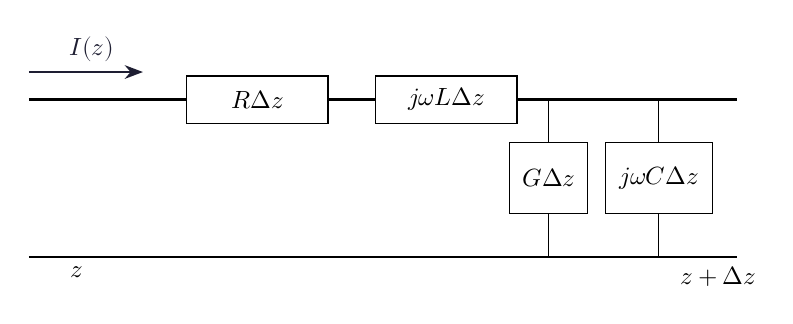
\begin{tikzpicture}[font=\small]
\draw[thick] (0,0)--(9,0) (0,2)--(2,2) (3.8,2)--(4.4,2) (6.2,2)--(9,2);
\draw (2,1.7) rectangle (3.8,2.3) node[pos=.5] {$R\Delta z$};
\draw (4.4,1.7) rectangle (6.2,2.3) node[pos=.5] {$j\omega L\Delta z$};
\draw (6.6,2)--(6.6,1.45) (6.6,.55)--(6.6,0) (8,2)--(8,1.45) (8,.55)--(8,0);
\draw (6.1,.55) rectangle (7.1,1.45) node[pos=.5] {$G\Delta z$};
\draw (7.32,.55) rectangle (8.68,1.45) node[pos=.5] {$j\omega C\Delta z$};
\draw[arrow] (0,2.35)--(1.45,2.35) node[above,pos=.55] {$I(z)$};
\node[below] at (.6,0) {$z$}; \node[below] at (8.75,0) {$z+\Delta z$};
\end{tikzpicture}
\end{tcolorbox}

Apply Kirchhoff's laws and take the limit:
\[
\begin{aligned}
V(z)-V(z+\Delta z)&=(R+j\omega L)\Delta z\,I(z),\\
I(z)-I(z+\Delta z)&\approx(G+j\omega C)\Delta z\,V(z),\\
\frac{dV}{dz}&=-Z'I,\qquad \frac{dI}{dz}=-Y'V ,
\end{aligned}
\]
where $Z'=R+j\omega L$ and $Y'=G+j\omega C$. The first equality is for the incremental circuit with its shunt at the right. The exact shunt voltage there is $V(z+\Delta z)$, replaced by $V(z)$ in the limit. The time-domain forms replace $j\omega$ by $\partial_t$ on the corresponding quantity.
\[
\begin{aligned}
V''&=Z'Y'V,\qquad I''=Z'Y'I,\\
V(z)&=V^+e^{-\gamma z}+V^-e^{\gamma z},\\
I(z)&=\frac{V^+}{Z_0}e^{-\gamma z}-\frac{V^-}{Z_0}e^{\gamma z}.
\end{aligned}
\]
Here $\gamma=\sqrt{Z'Y'}=\alpha+j\beta$ in $\mathrm{m^{-1}}$ and $Z_0=Z'/\gamma=\sqrt{Z'/Y'}$ in $\Omega$. Choose the passive forward branch. The minus sign in reflected current follows from $I=-V'/Z'$.
\begin{itemize}[leftmargin=*,itemsep=3pt]
\item \textbf{Lossless.} $R=G=0$, $Z_0=\sqrt{L/C}$, $\beta=\omega\sqrt{LC}$ and $v_p=1/\sqrt{LC}$.
\item \textbf{Low loss.} For $R\ll\omega L$ and $G\ll\omega C$, expand the square root to first order. Write $\gamma=j\omega\sqrt{LC}\sqrt{(1-jR/\omega L)(1-jG/\omega C)}$. With $\sqrt{1+x}\approx1+x/2$, $\alpha\approx R/(2Z_{00})+GZ_{00}/2$, $\beta\approx\omega\sqrt{LC}$ and $Z_{00}=\sqrt{L/C}$. The exact $Z_0$ may be complex.
\item \textbf{Distortionless case.} When $R/L=G/C$, $Z_0=\sqrt{L/C}$ and $\gamma=\sqrt{LC}(G/C+j\omega)$. Attenuation is independent of frequency and phase is linear under this ideal model.
\end{itemize}

\section{Termination, Impedance and Power}
\subsection{Reflection and standing waves}
Set load at $z=0$ and input at $z=-\ell$. At the load, $Z_L=Z_0(1+\Gamma_L)/(1-\Gamma_L)$ with $\Gamma_L=V^-/V^+$. Solve for $\Gamma_L$ and follow the phasors toward the generator:
\[
 \Gamma_L=\frac{Z_L-Z_0}{Z_L+Z_0},\qquad
 \Gamma_{\mathrm{in}}=\Gamma_L e^{-2\gamma\ell}.
\]
Short, open and matched loads give $-1$, $+1$ and 0 respectively. For a lossless line at distance $d$ from the load the relative phase is $\arg\Gamma_L-2\beta d$. Voltage maxima and minima occur when this is $0$ and $\pi$ modulo $2\pi$, respectively.
\begin{tcolorbox}[defbox,title={Voltage standing-wave ratio}]
The voltage standing-wave ratio (VSWR) is the voltage maximum divided by the voltage minimum. On a lossless line, $S=(1+|\Gamma_L|)/(1-|\Gamma_L|)$. Consecutive maxima are $\lambda/2$ apart and adjacent maximum and minimum are $\lambda/4$ apart. On appreciably lossy lines the ratio varies with position.
\end{tcolorbox}
\begin{tcolorbox}[examplebox,title={Complex load, VSWR and standing-wave positions}]
A lossless $50\,\Omega$ line ends in $Z_L=(75+j50)\,\Omega$. Distances $d$ are measured from the load toward the generator.
\[
\begin{aligned}
\Gamma_L&=\frac{25+j50}{125+j50}
  =\frac{(25+j50)(125-j50)}{125^2+50^2}\\
  &=0.3103+j0.2759=0.4152\angle41.6^\circ,\\
S&=\frac{1+0.4152}{1-0.4152}=2.42.
\end{aligned}
\]
For the nearest voltage maximum, $41.6^\circ-720^\circ d/\lambda=0$, so $d_{\max}=0.0578\lambda$. The first minimum is another $\lambda/4$ toward the generator, at $0.3078\lambda$. Use the magnitude of the reflection coefficient for VSWR and its phase for positions. About $82.8\%$ of the incident power reaches the load.
\end{tcolorbox}

\subsection{Exact and low-loss impedance transformation}
Substitute $\Gamma_{\mathrm{in}}$ into $Z_{\mathrm{in}}=Z_0(1+\Gamma_{\mathrm{in}})/(1-\Gamma_{\mathrm{in}})$, multiply numerator and denominator by $e^{\gamma\ell}(Z_L+Z_0)$ and group the exponential sums and differences. This gives
\[
 Z_{\mathrm{in}}=Z_0\frac{Z_L+Z_0\tanh(\gamma\ell)}{Z_0+Z_L\tanh(\gamma\ell)} .
\]
For lossless lines $\tanh(j\beta\ell)=j\tan\beta\ell$. For low-loss lines retain $\alpha\ell$ in the hyperbolic function if it is appreciable. Away from a pole, $\tanh(\alpha\ell+j\beta\ell)\approx j\tan\beta\ell+\alpha\ell\sec^2\beta\ell$ when the correction is small.
\begin{tcolorbox}[examplebox,title={Find characteristic impedance from open and short measurements}]
At the same frequency on the same uniform line section, measure the complex input impedances $Z_{\rm oc}$ and $Z_{\rm sc}$ by opening and shorting its far end. Taking $Z_L\to\infty$ and $Z_L=0$ gives
\[
\begin{aligned}
 Z_{\rm oc}&=Z_0\coth(\gamma\ell),&
 Z_{\rm sc}&=Z_0\tanh(\gamma\ell),\\
 Z_{\rm oc}Z_{\rm sc}&=Z_0^2 .
\end{aligned}
\]
Use the passive root. For $Z_{\rm sc}=j30\,\Omega$ and $Z_{\rm oc}=-j120\,\Omega$, $Z_0=60\,\Omega$. If the line is lossless and $0<\ell<\lambda/4$, then $\tan\beta\ell=30/60$ and $\ell/\lambda=\tan^{-1}(0.5)/(2\pi)=0.0738$ with the angle in radians.
\end{tcolorbox}

\begin{tcolorbox}[examplebox,title={Quarter-wave transformer and a low-loss comparison}]
To match a $100\,\Omega$ load to a $50\,\Omega$ feed, use a quarter-wave section with $Z_t=\sqrt{50(100)}=70.71\,\Omega$. Its lossless input is $Z_t^2/100=50\,\Omega$ at the design frequency.

For a $50\,\Omega$ line section itself feeding $100\,\Omega$, $\Gamma_L=1/3$. If $\ell=\lambda/4$ and $\alpha\ell=0.1$, take $Z_0\approx50\,\Omega$. Then $\Gamma_{\mathrm{in}}=-(1/3)e^{-0.2}=-0.2729$ and $Z_{\mathrm{in}}\approx28.56\,\Omega$. The lossless value is $25\,\Omega$.
\end{tcolorbox}
\subsection{Power transfer}
For peak phasors, $P=\operatorname{Re}(VI^*)/2$. At the load, use $V=V^++V^-$ and $I=(V^+-V^-)/Z_0$. For real $Z_0$ the product is
\[
 VI^*=\frac{|V^+|^2-|V^-|^2+
           V^-(V^+)^*-V^+(V^-)^*}{Z_0}.
\]
The two cross terms are a complex number minus its conjugate, so their real parts cancel. At the load this yields
\[
 P_L=\frac{|V^+|^2-|V^-|^2}{2Z_0}
 =\frac{|V^+|^2}{2Z_0}(1-|\Gamma_L|^2).
\]
Use $P_L/P_i=1-|\Gamma_L|^2$ and return loss $-20\log_{10}|\Gamma_L|$ in decibels. For complex $Z_0$ evaluate $\operatorname{Re}(VI^*)/2$ directly. Load matching removes reflection at that port. For maximum transfer from a fixed Thévenin generator, the load presented at the source reference plane must be the conjugate of its source impedance.
\begin{tcolorbox}[examplebox,title={Return loss, VSWR and delivered power}]
A $50\,\Omega$ lossless line delivers an incident $1\,\mathrm W$ to $Z_L=100\,\Omega$. $\Gamma_L=1/3$, $S=2$, return loss is $9.54\,\mathrm{dB}$ and $P_L=1(1-1/9)=0.889\,\mathrm W$.
\end{tcolorbox}

\section{Smith Chart and Matching}
\begin{tcolorbox}[defbox,title={Smith chart}]
A Smith chart maps normalized impedance to the complex voltage-reflection plane. Normalize $z_n=Z/Z_0=r+jx$ for a real $Z_0$. The centre is matched, the left rim is a short and the right rim an open.
\end{tcolorbox}
\subsection{Impedance and admittance grids}
For $\Gamma=u+jv$, use $z_n=(1+\Gamma)/(1-\Gamma)$. Taking real and imaginary parts and completing squares gives
\[
\begin{aligned}
 (u-r/(1+r))^2+v^2&=1/(1+r)^2,\\
 (u-1)^2+(v-1/x)^2&=1/x^2\qquad(x\ne0).
\end{aligned}
\]
Positive reactance lies above the real axis. The companion admittance grid is the impedance grid rotated by $180^\circ$ because $y_n=Y/Y_0=1/z_n$. On a single printed impedance grid, move to the diametrically opposite point to read the numerical $g+jb$. On a dual impedance/admittance chart, read the admittance grid at the original physical $\Gamma$ point. The change of grid alone is unrelated to line length.
\begin{tcolorbox}[tikzbox,title={Impedance Smith chart with a sample load},unbreakable]
\centering
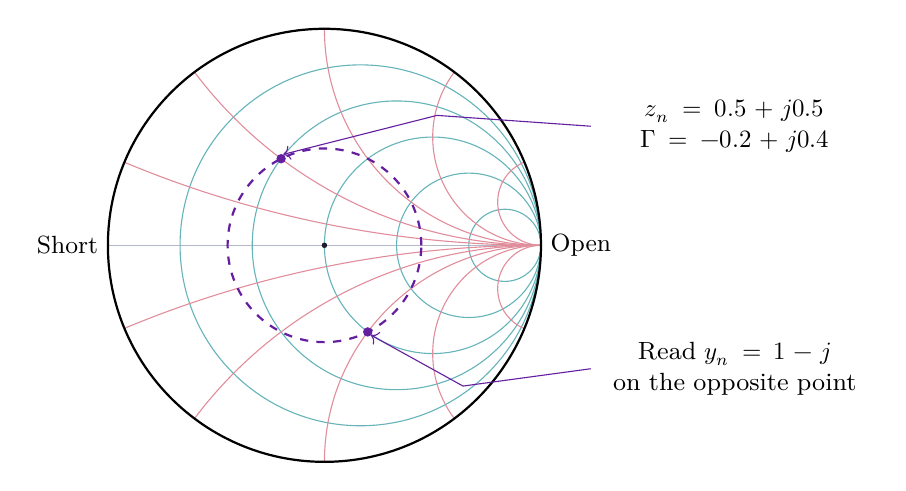
\begin{tikzpicture}[x=2.75cm,y=2.75cm,font=\small]
\begin{scope}
\clip (0,0) circle (1);
\draw[mgframe] (-1,0)--(1,0);
\foreach \r in {.2,.5,1,2,5}{
 \pgfmathsetmacro{\c}{\r/(1+\r)}
 \pgfmathsetmacro{\rad}{1/(1+\r)}
 \draw[myteal!60] (\c,0) circle (\rad);
}
\foreach \x in {.2,.5,1,2,5}{
 \pgfmathsetmacro{\rad}{1/\x}
 \draw[myred!50] (1,\rad) circle (\rad) (1,-\rad) circle (\rad);
}
\draw[dashed,mypurple,thick] (0,0) circle (.4472);
\end{scope}
\draw[thick] (0,0) circle (1);
\fill[mydark] (0,0) circle (1pt);
\fill[mypurple] (-.2,.4) circle (1.7pt) (.2,-.4) circle (1.7pt);
\node[align=center,text width=3.4cm,anchor=west] (load) at (1.23,.55) {$z_n=0.5+j0.5$\\$\Gamma=-0.2+j0.4$};
\draw[->,mypurple] (load.west)--(.52,.6)--(-.19,.42);
\node[align=center,text width=3.4cm,anchor=west] (adm) at (1.23,-.57) {Read $y_n=1-j$\\on the opposite point};
\draw[->,mypurple] (adm.west)--(.64,-.65)--(.215,-.415);
\node[left] at (-1,0) {Short}; \node[right] at (1,0) {Open};
\end{tikzpicture}
\end{tcolorbox}
\begin{enumerate}[leftmargin=*,itemsep=3pt]
\item Plot the normalized load at the intersection of its constant-$r$ circle and constant-$x$ arc.
\item Draw a constant-$|\Gamma|$ circle about the centre for a lossless line. Move clockwise toward the generator through $2\beta\ell$, or counterclockwise toward the load. A complete turn corresponds to $\lambda/2$.
\item Read the intersection with the new resistance and reactance curves. Multiply by $Z_0$ for ohms. With loss the point spirals inward on a generatorward move.
\item For $z_n=0.5+j0.5$ the illustrated point gives $|\Gamma|=\sqrt{0.2}$, so VSWR is $2.618$. A $\lambda/8$ move rotates clockwise by $90^\circ$, giving $\Gamma_{\mathrm{in}}=0.4+j0.2$ and $z_{\mathrm{in}}=2+j1$.
\end{enumerate}

\subsection{Single-stub matching and line sections as elements}
For a shunt stub, translate along the main line to a point with normalized admittance $1+jb$. Then add a stub of admittance $-jb$. An ideal stub carries reactive current and absorbs zero average power. Use the same real $Z_0$ for the main line and stub in the following example.
\begin{tcolorbox}[examplebox,title={Shunt shorted-stub match in admittance form}]
Take $Z_L=25\,\Omega$ on $Z_0=50\,\Omega$. Then $y_L=2$. At distance $d$ toward the generator, put $t=\tan\beta d$.
\[
 y(d)=\frac{2+jt}{1+j2t}
      =\frac{2(1+t^2)-j3t}{1+4t^2}.
\]
Set the real part to 1. This gives $t^2=1/2$. Choose $t=+0.7071$, hence $d=0.0980\lambda$, $y(d)=1-j0.7071$. A shorted stub gives $y_s=-j\cot(\beta\ell_s)$. Choose $\beta\ell_s=125.26^\circ$, or $\ell_s=0.3480\lambda$, so $y(d)+y_s=1$.
\end{tcolorbox}
\par\vspace{6pt}\noindent
\begin{tabularx}{\linewidth}{|B{4cm}|Y|}\hline
Lossless section & Input impedance or application \\ \hline
Short-circuit stub & $jZ_0\tan\beta\ell$. Electrically short: $j\omega L\ell$, an inductance. \\ \hline
Open-circuit stub & $-jZ_0\cot\beta\ell$. Electrically short: $1/(j\omega C\ell)$, a capacitance. \\ \hline
Quarter wavelength & $Z_0^2/Z_L$, so open and short exchange roles. A real load transforms through a suitable section impedance. \\ \hline
Half wavelength & Repeats $Z_L$ on a lossless line. Rotation on the Smith chart is a full turn. \\ \hline
\end{tabularx}


\newpage
\begin{center}
  {\large\bfseries\color{myred} Quick Revision --- Module 3}\\[3pt]
  {\small\color{mydark} Transmission Lines and Smith Chart $|$ EC501}
\end{center}
\noindent{\color{myred}\rule{\linewidth}{1.2pt}}
\begin{tcolorbox}[formulabox,title={Key Formulas at a Glance}]
\renewcommand{\arraystretch}{1.35}
\begin{tabularx}{\linewidth}{B{5.0cm}Y}
Distributed model & $\gamma=\sqrt{Z'Y'}$ and $Z_0=\sqrt{Z'/Y'}$ \\[3pt]
Voltage reflection & $\Gamma_L=(Z_L-Z_0)/(Z_L+Z_0)$ \\[3pt]
Input reflection & $\Gamma_{\mathrm{in}}=\Gamma_Le^{-2\gamma\ell}$ \\[3pt]
Standing-wave ratio & $(1+|\Gamma|)/(1-|\Gamma|)$ on a lossless line \\[3pt]
Real-impedance power & $P_L=P_i(1-|\Gamma_L|^2)$ for real $Z_0$ \\[3pt]
Quarter-wave match & $Z_t=\sqrt{Z_{\rm feed}R_L}$ for a resistive load \\[3pt]
\end{tabularx}
\end{tcolorbox}
\begin{tcolorbox}[defbox,title={One-Line Definitions}]
\textbf{Characteristic impedance.} Ratio of forward voltage to forward current on a uniform line.\par
\textbf{Reflection coefficient.} Complex ratio of reverse to forward voltage at a specified reference plane.\par
\textbf{Stub.} An open- or short-terminated section used as a frequency-dependent reactance or susceptance.\par
\end{tcolorbox}
\begin{tcolorbox}[exambox,title={Frequently Asked / Viva Questions}]
\begin{enumerate}[topsep=0pt, label=\textbf{Q\arabic*.}, itemsep=5pt]
\item \Q{What is the sign of reverse current?}
It is the negative of reverse voltage divided by $Z_0$ with current referenced toward the load.
\item \Q{When is a line lossless?}
When its series resistance and shunt conductance per metre are both zero.
\item \Q{How is a line's voltage equation obtained?}
Differentiate $V'=-Z'I$ and substitute $I'=-Y'V$.
\item \Q{What does matching at the load accomplish?}
It makes $\Gamma_L=0$.
\item \Q{What is the VSWR for an ideal open?}
Infinite on a lossless line because the voltage minimum is zero.
\item \Q{How far apart are adjacent voltage maxima?}
Half a wavelength.
\item \Q{Why does the load point rotate clockwise toward the generator?}
Its phase changes by $-2\beta\ell$.
\item \Q{How is admittance read on an impedance-only chart?}
Read the point diametrically opposite the normalized impedance.
\item \Q{What must the main-line admittance be for a shunt-stub match?}
Its normalized conductance must be one before stub susceptance cancels the imaginary part.
\item \Q{Why is a quarter-wave match frequency selective?}
The section has the required electrical length only at specified frequencies.
\end{enumerate}
\end{tcolorbox}
\begin{tcolorbox}[tikzbox,title={Summary comparison}]
\begin{tabularx}{\linewidth}{|B{4cm}|Y|}\hline
\textbf{Case} & \textbf{What to use} \\ \hline
Lossless movement & Clockwise along constant $|\Gamma|$ toward the generator. \\ \hline
Lossy movement & Clockwise and inward toward the generator. \\ \hline
Shunt stub & Match conductance first, then cancel susceptance. \\ \hline
\end{tabularx}
\end{tcolorbox}
\end{document}
